\section{Architecture and Implementation}
\label{sec:architecture}

%%%%%%%%%%%%%%%%%%%%%%%%%%%%%%%%%%%%%%%%%%%%%%%%%%%%%%%%%%%%%%%%%%%%%%%%%%%%%%%%%%%%%%%
% Intro to arch
%%%%%%%%%%%%%%%%%%%%%%%%%%%%%%%%%%%%%%%%%%%%%%%%%%%%%%%%%%%%%%%%%%%%%%%%%%%%%%%%%%%%%%%

To simplify and address concerns outlined in the previous section we introduce two
major changes. We introduce safe collections, an abstraction that encapsulates
a data-set and the set of policies that govern it's use. Seconondly, in order to separate
administative responsibilities pertaining to the safe-collection from the infrastructure
admins, we create a new class of privileged users called Stewards. In this design, administrators
create a safe collection and hand over all administrative privileges to the stewards. This transfers
all administrative responsibilities regarding access and export of data to the stewards who now take
ownership and responsibility for the safe collection.

\subsection{Safe Collection}

Data-sets come with various levels of sensitivity and the selecting protocols to ensure adequate security
requires a case-by-case treatement. To closely integrate such policies with the data-set we have created
safe-collections. Our implementation supports a range of protocols to be enforced on the data-set in
three key areas: Access control, Export control and Link control. These controls can be described through a
document.

\begin{figure}
  \center
  %\includegraphics[width=0.45\textwidth]{figures/arch.pdf}
  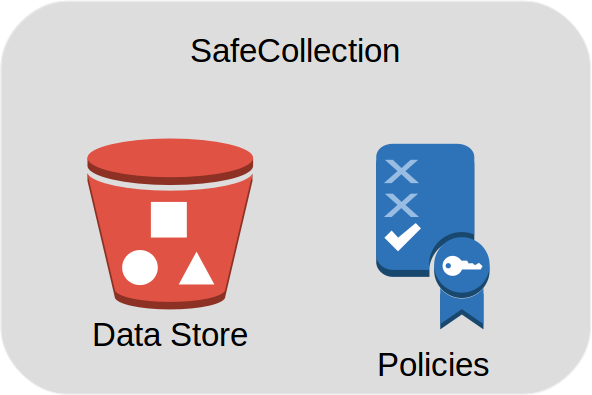
\includegraphics[width=0.45\textwidth]{figures/safecollection.png}
  \caption{Safe collection schema}
  \label{fig:safe_schema}
  \vspace{-1.5em}
\end{figure}

\begin{figure}
  \center
  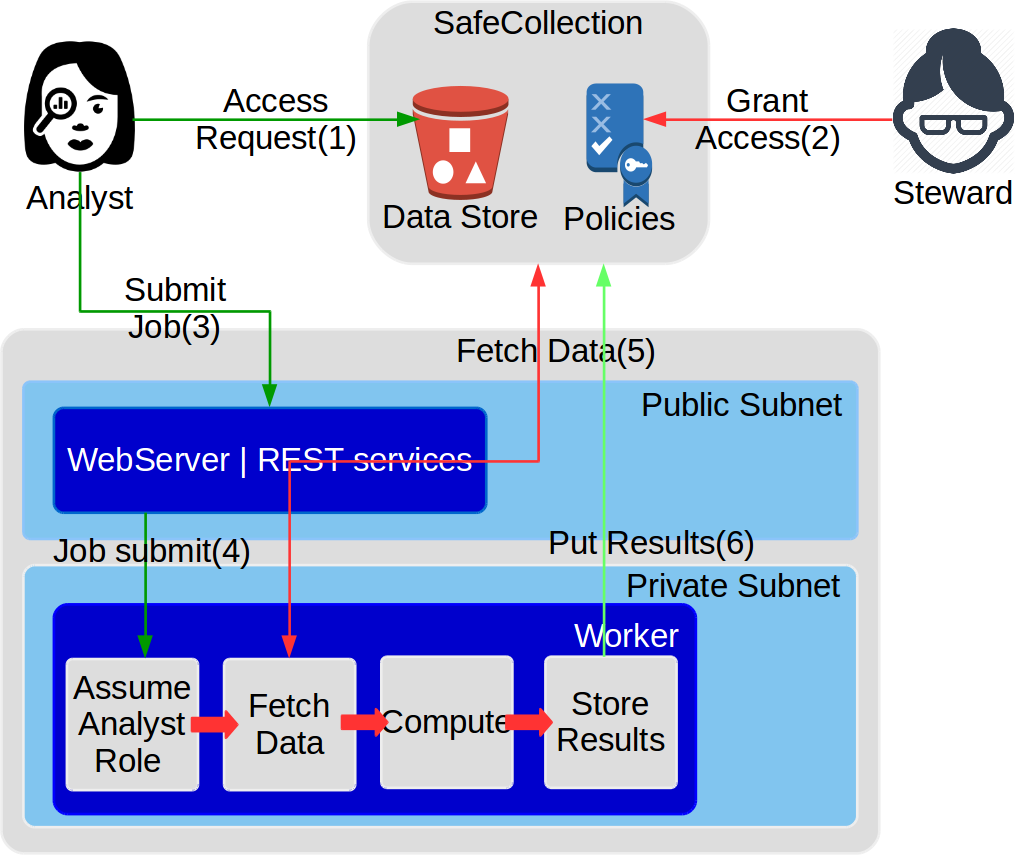
\includegraphics[width=0.45\textwidth]{figures/safe_flow.png}
  \caption{Safe collection schema}
  \label{fig:flow1}
  \vspace{-1.5em}
\end{figure}


\begin{figure}
  \center
  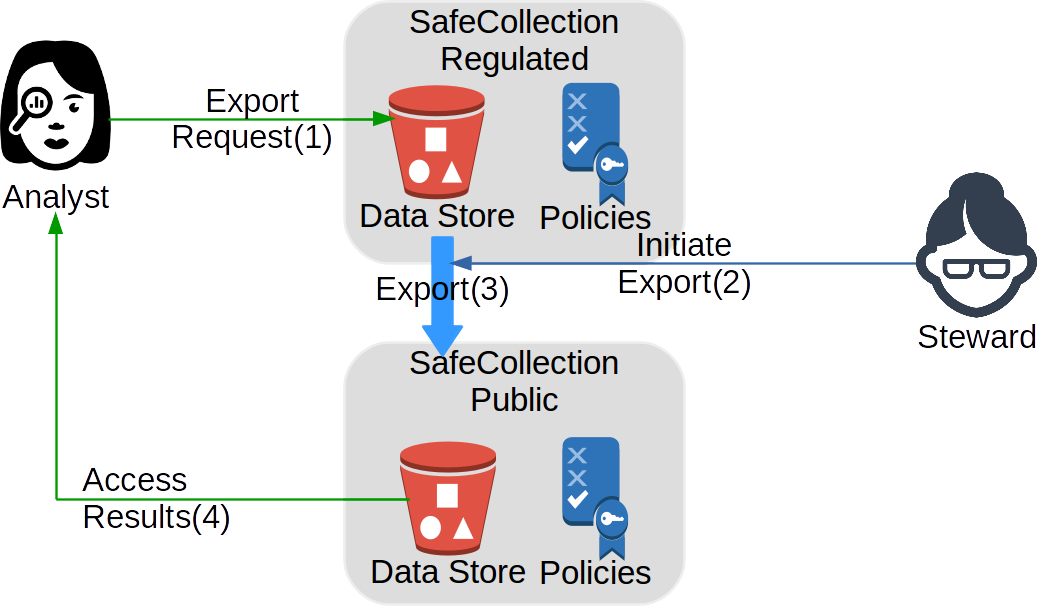
\includegraphics[width=0.45\textwidth]{figures/export_flow.png}
  \caption{Safe collection schema}
  \label{fig:flow2}
  \vspace{-1.5em}
\end{figure}









